\section{Nonlinear Parameter identification}
\label{SubSecEstimation}

The behavior of the complete water distribution system is governed by the previously derived model. Certain parameters of the system are either unknown or can vary significantly from the assumed design values. Furthermore, the obtained model of the system gives nonlinear relations between flows and pressures in each individual components. 
\\  
In case of the valves, the conductivity function is dependent on the OD, therefore the parameter of these elements are considered to be known. The centrifugal pumps are fully described by their models and by the coefficients provided by the manufacturer. The hydraulic capacity is also considered as known in case of the WT. However, parameters in the model of the pipes are uncertain. Even though the necessary friction parameters can be found in the data sheet provided by the manufacturer. These values are only acceptable for new pipes, as over time material can build up on the inside of the pipes, since the laboratory setup to a large extent is built from PEX/PEM (plastic) pipes. Furthermore, the physical parameters of the pipe volumes are assumed to be known to an accuracy where there is not any benefits from estimating it. Therefore the inertia matrix is known.  

The aim of the system identification in case of the water distribution system is to estimate the missing parameters which describe the frictions and form losses in the pipes. Therefore, defining the additional pressure losses and thus obtain a model that precisely describes the system. This is especially important in order to ensure correct behavior when applying the MPC, which will be based on the parameter estimated model to the actual system. Due to these considerations, the importance of obtaining accurate parameters is additionally essential in order to setup a simulation that represents the real test setup. 

%The parameter estimation is introduced for two different cases with different approaches. One being an estimation method with the model being kept non-linear, the other being a method where the model is  linearized before the estimation. 

The block diagram of a general parameter identification method is shown in \figref{fig:parame_block}. 

\begin{figure}[H]
\centering
\usetikzlibrary{arrows}
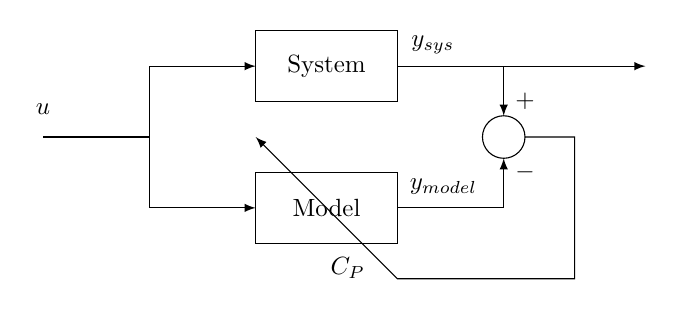
\begin{tikzpicture} [scale=0.9,transform shape]

\draw  (3,-1.5) rectangle (5,-2.5);
\node at (4,-2) {Model};

\draw  (3,0.5) rectangle (5,-0.5);
\node at (4,0) {System};

\node at (6.8,-1.5) {$-$};
\node at (5.5,0.3) {$y_{sys}$};
\node at (5.65,-1.7) {$y_{model}$};
\node at (4.3,-2.85) {$C_P$};
\node at (0,-0.6) {$u$};
\node at (6.8,-0.5) {$+$};

\draw  (6.5,-1) ellipse (0.3 and 0.3);

\draw [-latex](5,0) -- (8.5,0);
\draw [-latex](6.5,0) -- (6.5,-0.7);
\draw [-latex](1.5,-1) -- (1.5,0) -- (3,0);
\draw [-latex](1.5,-1) -- (1.5,-2) -- (3,-2);
\draw (0,-1) -- (1.5,-1);
\draw [-latex](5,-2) -- (6.5,-2) -- (6.5,-1.3);
\draw [-latex](6.8,-1) -- (7.5,-1) -- (7.5,-3) -- (5,-3) -- (3,-1);

\end{tikzpicture}% 
\caption{Parameter identification block diagram. }
\label{fig:parame_block}
\end{figure}

As it is shown in the figure, the measurements from the real life system are compared to the output of the simulation introducing the same input for both systems. In the figure, $C_{res}$ denotes the unknown resistance parameters.

In order to obtain measurements from the real life test setup, the system has to be excited by various input signals. The inputs to the system are the input signals to the pumps, however in case of the parameter estimation the OD of the valves are also considered as inputs. Therefore, it is reasonable to reformulate the equation describing the network in \eqref{ParatModelFinal} into such a form where the terms for the inputs and states are isolated. Recalling \eqref{isolateZ}, the system equation is in such a form, except that the input only considers the two main and two PMA pumps: 

\begin{equation}
\bm{B} \bm{J} \bm{B^T} \bm{\dot{z}} = - \bm{B} f(\bm{B^T}\bm{z}, \bm{OD}) + \bm{B}\tilde{\alpha} (\bm{\omega},\bm{B^T}\bm{z}) 
 %\pmb{B}\pmb{J {B}}^T \pmb{\dot{z}} = \pmb{B} g(\pmb{B}^T \pmb{z})+ \pmb{B} u(\pmb{\omega},\pmb{k_v	}, \pmb{B}^T \pmb{z})
 \label{InputOutputmodel}
\end{equation}

Reformulating \eqref{InputOutputmodel} such that all valves and pumps are isolated in the input, the following yields:

\begin{equation}
\bm{B} \bm{J} \bm{B^T} \bm{\dot{z}} = - \bm{B} \tilde f(\bm{B^T}\bm{z}) + \bm{B} u(\bm{\omega},\bm{B^T}\bm{z},\bm{OD}) 
 %\pmb{B}\pmb{J {B}}^T \pmb{\dot{z}} = \pmb{B} g(\pmb{B}^T \pmb{z})+ \pmb{B} u(\pmb{\omega},\pmb{k_v  }, \pmb{B}^T \pmb{z})
 \label{InputOutputmodel2}
\end{equation}

where the vectorfield $u(\bm{\omega},\bm{B^T}\bm{z},\bm{OD})$ contains all the functions for the elements, which are dependent on the inputs. The vectorfield $\tilde f(\bm{B^T}\bm{z})$ describes the rest of the resistance terms which are responsible for the pressure drops in the network. Although $u(\cdot)$ takes the inputs as $\omega$ and $OD$, during the estimation and the control, the inputs to the pumps are specified as pressure differences, $\Delta p$.

In the system, outputs are defined as differential pressures according to the available sensors on the test setup. From the system setup $8$ different relative pressures can be measured. Following the notation of \figref{systemdiagram}, sensors are placed in: 
$n_2$, $n_4$, $n_5$, $n_7$, $n_{10}$, $n_{11}$, $n_{15}$, and  $n_{16}$. During the parameter identification, these measurements are compared to the output from the simulation and the parameters are varied until the model fits the data.

It is important to point out that the estimation is applied for steady-state, since the unknown parameters are the resistances and form losses. The inertia and the capacitance only affect the dynamics, therefore have no influence during steady-state. The inertia of the pipes, and the capacitance of the WT are considered as known parameters. 

Taking the steady-state into account, the system equation for the nonlinear parameter estimation can be rewritten as: 

\begin{equation}
 0 = \underbrace {-\bm{B} \tilde f(\bm{B^T}\bm{z}) + \bm{B} u(\bm{\omega},\bm{B^T}\bm{z},\bm{OD}) }_{\mathcal{\bm{X}}}
 \label{InputOutputmodel_steadystate}
\end{equation}

The aim of the parameter identification is to obtain a minimum difference between the outputs by adjusting the parameters of the resistance terms. The general parameter estimation problem is a minimization problem with the following objective function over the variable $\bm{z}$: 

%\begin{equation}
%
%  \sum_{i=1}^{n}\Big(g_{\pmb(Cp)}(\pmb{B}^T \pmb{z}_i)\Big)
%
%\label{ObjectiveFunction}
%\end{equation}
\todo{Explain this better and correct notation!!!}
 \begin{equation}
 \min_{z} \Big(\mathcal{\bm{X}}^T \mathcal{\bm{X}} + \big(\bm{y_{s}(B^T z)} - \bm{y_{m}(B^T z)} \big)^T  \big(\bm{ y_{s}(B^T z)} - \bm{ y_{m}(B^T z)\big)}\Big)
  \label{ObjectiveFunction11}
 \end{equation}
 
\begin{minipage}[t]{0.20\textwidth}
Where\\
\hspace*{8mm} $\bm{y_{s}(B^T z)}$ \\
\hspace*{8mm} $\bm{y_{m}(B^T z)}$ \\
\hspace*{8mm} $\mathcal{\bm{X}}$ 
\end{minipage}
\begin{minipage}[t]{0.68\textwidth}
\vspace*{2mm}
is the vector of pressure measurements on the system,\\
is the vector of outputs in the model, \\
is the term defined in \eqref{ObjectiveFunction11}.
\end{minipage}
\begin{minipage}[t]{0.10\textwidth}
\vspace*{2mm}
\textcolor{White}{te}$\unit{bar}$
\textcolor{White}{te}$\unit{bar}$
\textcolor{White}{te}$\unit{bar}$
\end{minipage}
\subsection{Measurements on the test setup}

On the system setup, \figref{systemdiagram}, $8$ different relative pressures can be measured. The measurements obtained from the pressure sensors 
placed in these nodes are relative to the atmospheric pressure. In order to compare the measurements from the system setup and the data 
obtained from the simulation in Matlab, an atmospheric pressure node, $n_1$, is set as reference point. Thus, the relation between the measured 
outputs and the reference point can be set, resulting in:
%\todo{Now we write $\Delta p$ or dP as Dp. Pls find one way of writing this. Furthermore, what is all the Cxx ? We need a where list or something similar. }

\text{\underline{Node 2}} 
\vspace{4mm}
\begin{equation}
    y_1 = \Delta p_{C2} 
\end{equation}

\text{\underline{Node 7}}
\vspace{4mm}
\begin{equation}
   y_2 = \Delta p_{C16} 
 \end{equation}

\text{\underline{Node 4}}
\vspace{4mm}
\begin{equation}
    y_3 = \Delta p_{C18} + \Delta p_{C19} + \Delta p_{C23} + \Delta p_{C24} 
\end{equation}

\text{\underline{Node 5}}
\vspace{4mm}
\begin{equation}
    y_4 = \Delta p_{C25} + \Delta p_{C26} + \Delta p_{C30} + \Delta p_{C31}  
\end{equation}

\text{\underline{Node 10}}
\vspace{4mm}
\begin {equation}
    y_5 = \Delta p_{C24}
\end{equation}

\text{\underline{Node 11}}
\vspace{4mm}
\begin {equation}
    y_6 = \Delta p_{C20} + \Delta p_{C21} 
\end{equation}

\text{\underline{Node 15}}
\vspace{4mm}
\begin {equation}
   y_7 = \Delta p_{C31}
\end{equation}

\text{\underline{Node 16}}
\vspace{4mm}
\begin {equation}
   y_8 = \Delta p_{C28} + \Delta p_{C27} 
\end{equation}

 
\subsection{Estimation method} 
\label{MatlabScript}

In order to carry out the parameter estimation of the water distribution, Matlab NonLinear Grey Box (MNGB) toolbox\cite{MatlabGreyBox}, is used. This toolbox 
estimates previously defined coefficients of nonlinear differential equations, to fit with the desired data. 
Thereby, a nonlinear model has to be designed to complete the simulation. 

The comparison between the test setup measurements and the estimated data is done with Matlab function \textit{compare}. Together with the comparison 
plot, the normalized root mean square (NRMSE) measure is also added which measures the goodness of the fit. This fit is calculated as a percentage \cite{MatlabFit} using:

\begin{equation}
  fit = 100 \bigg(1 - \frac{||y_s - y_m||}{||y_s - mean(y_s)||}\bigg)
  \label{fitequation}
\end{equation} 

\begin{minipage}[t]{0.20\textwidth}
Where\\
\hspace*{8mm} $y_s$ \\
\hspace*{8mm} $y_m$ \\
\end{minipage}
\begin{minipage}[t]{0.68\textwidth}
\vspace*{2mm}
is the validation data, the outcome of the measurement \\
is the output of the model\\
\end{minipage}
\begin{minipage}[t]{0.10\textwidth}
\vspace*{2mm}
\textcolor{White}{te}$\unit{Bar}$
\textcolor{White}{te}$\unit{Bar}$
\end{minipage}

\subsection{Nonlinear Estimation Outcomes} 
\label{NonLiOutcome}
The results of the nonlinear parameter estimation are shown in \appref{NonLinResults}. It is obvious that the estimation has been unsuccessful, seeing 
that the model and the measured data follow different behaviors. This might be due to the incapability to excite the system sufficiently in order to estimated the pipe parameters correctly due to limited information in the measured data. Moreover, the dynamics of the valves are slower in comparison with dynamics of the pipes, resulting in the information of the pipes being hidden into the dynamics of the valves. Thus preventing the estimation process from obtaining the correct values for the resistance as only the valve dynamic are present in the output data.

An alternative could be to only use the pumps as inputs without affecting
the valves dynamics. However in order to obtain accurate values for the parameters, different scenarios have to be simulated which include varying the water consumption 
of the end-users as the pumps cannot excite the system sufficiently on there own. 

Therefore, after seeing that the nonlinear approach is not suitable to estimate the unknown parameters for this test setup, the model will be linearized in order to preform a linear parameter estimation.